\clearpage


\section{Validation of the $\bar{\nu}/\nu$ joint analysis with Run 1-7 update}
\label{sec:validation_run17}

The major update to the analysis is the number of POT, 
i.e. 
\TotalPotNuRunOneSeven{} POT for neutrino mode
and
\TotalPotNuBarRunOneSeven{} POT for antineutrino mode. 

Other minor updates are the new BANFF covariance matrix.
The BANFF fit was not performed again on the full ND280 Run 1-7 data set
and the Run 7 Super-K flux covariance matrix (pre-BANFF fit) was added in quadrature
to the Run 1-6 covariance matrix.
Furthermore the flux tuning was updated in order to account for the Run 7.
However both updates give a very small effect and will not change significantly the systematic
uncertainties and event rate in the analysis.

%
% Event rate and systematic uncertainties
%

\subsection{Prediction of event rate and effect of systematic uncertainties}
\label{sec:event_rate_syst_run17}


% N.B.: Spectra are in the results section


In \cref{tab:events_1rmu_Asimov_A_Run17} - \ref{tab:events_rhc1re_Asimov_A_Run17} 
the expected number of events for the Run 1-7 collected statistic is shown for the Asimov data set A.
In appendix~\ref{app:events_run17} the expected event rate for each Super-K samples is shown for the Asimov data set B.

\input{tables/Run17/validation_1rmu_Asimov_A.tex}
\input{tables/Run17/validation_1re_Asimov_A.tex}
\input{tables/Run17/validation_rhc1rmu_Asimov_A.tex}
\input{tables/Run17/validation_rhc1re_Asimov_A.tex}

\clearpage

In \cref{tab:nsk_systematic_table_summary_joint_asimov_A_fhc_mulike_Run17} - 
\ref{tab:nsk_systematic_table_summary_joint_asimov_A_rhc_elike_Run17}
the effect of each source of systematic uncertainty on the total number of expected events in each sample is shown
for Asimov data set A.

In \cref{tab:ratio_systematic_table_summary_asimov_A_Run17} 
the effect of each source of systematic uncertainty on the ratio between the number of events in 
neutrino and antineutrino mode samples is shown for Asimov data set A.

This tables can be directly compared with \cref{tab:nsk_systematic_table_summary_joint_asimov_A_fhc_mulike} -
\ref{tab:ratio_systematic_table_summary_asimov_A} of the Run 1-6 data set analysis.

In appendix~\ref{app:systematics_run17} the effect of each source of systematic uncertainty 
is shown for Asimov data set B.

Given the minor change in the BANFF covariance matrix, the uncertainties are very similar
the Run 1-6 analysis ones.

\input{./tables/Run17/nsk_systematic_table_summary_Asimov_A.tex}


\clearpage



In \cref{fig:spectra_systematic_Asimov_A_run17} - \ref{fig:flux_xsec_envelope_Asimov_A_run17}
the systematic error envelope as well as the fractional error as a function of the
neutrino reconstructed energy is shown for each source of systematic uncertainty
as well as for all the systematic uncertainties. 
The spectra correspond to the oscillation parameters of the Asimov data set A.


\begin{figure*}[htb]
\center
%fhc mu-like
\begin{subfigure}[b]{0.49\textwidth} \centering
\includegraphics[width=0.9\textwidth]{joint_plots/systematics/Run17/Asimov_A_1Rmuoscillated_all_envelope.eps} 
\caption{Muon-like, neutrino mode}
\end{subfigure}
\begin{subfigure}[b]{0.49\textwidth} \centering
\includegraphics[width=0.9\textwidth]{joint_plots/systematics/Run17/Asimov_A_1Rmuoscillated_all_envelope_ratio.eps} \\
\caption{Muon-like, neutrino mode}
\end{subfigure}
%rhc mu-like
\begin{subfigure}[b]{0.49\textwidth} \centering
\includegraphics[width=0.9\textwidth]{joint_plots/systematics/Run17/Asimov_A_RHC1Rmuoscillated_all_envelope.eps} %\\ 
\caption{Muon-like, antineutrino mode}
\end{subfigure}
\begin{subfigure}[b]{0.49\textwidth} \centering
\includegraphics[width=0.9\textwidth]{joint_plots/systematics/Run17/Asimov_A_RHC1Rmuoscillated_all_envelope_ratio.eps} \\ 
\caption{Muon-like, antineutrino mode}
\end{subfigure}
%fhc e-like
\begin{subfigure}[b]{0.49\textwidth} \centering
\includegraphics[width=0.9\textwidth]{joint_plots/systematics/Run17/Asimov_A_1Reoscillated_all_envelope.eps} 
\caption{Electron-like, neutrino mode}
\end{subfigure}
\begin{subfigure}[b]{0.49\textwidth} \centering
\includegraphics[width=0.9\textwidth]{joint_plots/systematics/Run17/Asimov_A_1Reoscillated_all_envelope_ratio.eps} 
\caption{Electron-like, neutrino mode}
\end{subfigure}
%rhc e-like
\begin{subfigure}[b]{0.49\textwidth} \centering
\includegraphics[width=0.9\textwidth]{joint_plots/systematics/Run17/Asimov_A_RHC1Reoscillated_all_envelope.eps} 
\caption{Electron-like, antineutrino mode}
\end{subfigure}
\begin{subfigure}[b]{0.49\textwidth} \centering
\includegraphics[width=0.9\textwidth]{joint_plots/systematics/Run17/Asimov_A_RHC1Reoscillated_all_envelope_ratio.eps} 
\caption{Electron-like, antineutrino mode}
\end{subfigure}
\caption {
Error envelopes (left) and fractional errors (right) for the reconstructed neutrino energy spectrum
for all the systematic parameters.
10k toy MC experiments are generated for the Asimov data set A shown in \cref{tab:osc_params_joint_asimov}
with randomized systematic parameters, taking into account their correlations.
Since the parameters $\delta_{CP}$, $\theta_{23}$ and $\Delta m^2_{32}$ ($\Delta m^2_{13}$) and mass hierarchy
will be measured,
only the uncertainty on 
$\sin^2 \theta_{13}$,
$\sin^2 \theta_{12}$
and 
$\Delta m^2_{21}$ 
are taken into account.
BANFF tuned MC templates are used. 
The distributions correspond to the collected statistics in the full Run 1-7 data set.
The changes due to the Run 1-7 flux and covariance matrix updates are applied.
}
\label{fig:spectra_systematic_Asimov_A_run17}
\end{figure*}



%%%% Single systematic sources of Asimov A


\begin{figure*}[htb]
\center
%fhc mu-like
\begin{subfigure}[b]{0.49\textwidth} \centering
\includegraphics[width=0.9\textwidth]{joint_plots/systematics/Run17/Asimov_A_1Rmuoscillated_Osc_param_envelope.eps}
\caption{Muon-like, neutrino mode}
\end{subfigure}
\begin{subfigure}[b]{0.49\textwidth} \centering
\includegraphics[width=0.9\textwidth]{joint_plots/systematics/Run17/Asimov_A_1Rmuoscillated_Osc_param_envelope_ratio.eps} 
\caption{Muon-like, neutrino mode}
\end{subfigure}
%rhc mu-like
\begin{subfigure}[b]{0.49\textwidth} \centering
\includegraphics[width=0.9\textwidth]{joint_plots/systematics/Run17/Asimov_A_RHC1Rmuoscillated_Osc_param_envelope.eps} \\ 
\caption{Muon-like, antineutrino mode}
\end{subfigure}
\begin{subfigure}[b]{0.49\textwidth} \centering
\includegraphics[width=0.9\textwidth]{joint_plots/systematics/Run17/Asimov_A_RHC1Rmuoscillated_Osc_param_envelope_ratio.eps} \\ 
\caption{Muon-like, antineutrino mode}
\end{subfigure}
%fhc e-like
\begin{subfigure}[b]{0.49\textwidth} \centering
\includegraphics[width=0.9\textwidth]{joint_plots/systematics/Run17/Asimov_A_1Reoscillated_Osc_param_envelope.eps} 
\caption{Electron-like, neutrino mode}
\end{subfigure}
\begin{subfigure}[b]{0.49\textwidth} \centering
\includegraphics[width=0.9\textwidth]{joint_plots/systematics/Run17/Asimov_A_1Reoscillated_Osc_param_envelope_ratio.eps}
\caption{Electron-like, neutrino mode}
\end{subfigure}
%rhc e-like
\begin{subfigure}[b]{0.49\textwidth} \centering
\includegraphics[width=0.9\textwidth]{joint_plots/systematics/Run17/Asimov_A_RHC1Reoscillated_Osc_param_envelope.eps}
\caption{Electron-like, antineutrino mode}
\end{subfigure}
\begin{subfigure}[b]{0.49\textwidth} \centering
\includegraphics[width=0.9\textwidth]{joint_plots/systematics/Run17/Asimov_A_RHC1Reoscillated_Osc_param_envelope_ratio.eps} 
\caption{Electron-like, antineutrino mode}
\end{subfigure}
\caption {
Error envelopes (left) and fractional errors (right) for the reconstructed neutrino energy spectrum
as a result of the oscillation systematic parameters.
10k toy MC experiments are generated for the Asimov data set A shown in \cref{tab:osc_params_joint_asimov}
with randomized systematic parameters, taking into account their correlations.
Since the parameters $\delta_{CP}$, $\theta_{23}$ and $\Delta m^2_{32}$ ($\Delta m^2_{13}$) and mass hierarchy
will be measured,
only the uncertainty on 
$\sin^2 \theta_{13}$,
$\sin^2 \theta_{12}$
and 
$\Delta m^2_{21}$ 
are taken into account.
BANFF tuned MC templates are used. 
The distributions correspond to the collected statistics in the full Run 1-7 data set.
The changes due to the Run 1-7 flux and covariance matrix updates are applied.
}
\label{fig:Osc_envelope_Asimov_A_run17}
\end{figure*}


\begin{figure*}[htb]
\center
%fhc mu-like
\begin{subfigure}[b]{0.49\textwidth} \centering
\includegraphics[width=0.9\textwidth]{joint_plots/systematics/Run17/Asimov_A_1Rmuoscillated_SKDet_FSI_envelope.eps} 
\caption{Muon-like, neutrino mode}
\end{subfigure}
\begin{subfigure}[b]{0.49\textwidth} \centering
\includegraphics[width=0.9\textwidth]{joint_plots/systematics/Run17/Asimov_A_1Rmuoscillated_SKDet_FSI_envelope_ratio.eps} 
\caption{Muon-like, neutrino mode}
\end{subfigure}
%rhc mu-like
\begin{subfigure}[b]{0.49\textwidth} \centering
\includegraphics[width=0.9\textwidth]{joint_plots/systematics/Run17/Asimov_A_RHC1Rmuoscillated_SKDet_FSI_envelope.eps} \\ 
\caption{Muon-like, antineutrino mode}
\end{subfigure}
\begin{subfigure}[b]{0.49\textwidth} \centering
\includegraphics[width=0.9\textwidth]{joint_plots/systematics/Run17/Asimov_A_RHC1Rmuoscillated_SKDet_FSI_envelope_ratio.eps} \\ 
\caption{Muon-like, antineutrino mode}
\end{subfigure}
%fhc e-like
\begin{subfigure}[b]{0.49\textwidth} \centering
\includegraphics[width=0.9\textwidth]{joint_plots/systematics/Run17/Asimov_A_1Reoscillated_SKDet_FSI_envelope.eps} 
\caption{Electron-like, neutrino mode}
\end{subfigure}
\begin{subfigure}[b]{0.49\textwidth} \centering
\includegraphics[width=0.9\textwidth]{joint_plots/systematics/Run17/Asimov_A_1Reoscillated_SKDet_FSI_envelope_ratio.eps} 
\caption{Electron-like, neutrino mode}
\end{subfigure}
%rhc e-like
\begin{subfigure}[b]{0.49\textwidth} \centering
\includegraphics[width=0.9\textwidth]{joint_plots/systematics/Run17/Asimov_A_RHC1Reoscillated_SKDet_FSI_envelope.eps} 
\caption{Electron-like, antineutrino mode}
\end{subfigure}
\begin{subfigure}[b]{0.49\textwidth} \centering
\includegraphics[width=0.9\textwidth]{joint_plots/systematics/Run17/Asimov_A_RHC1Reoscillated_SKDet_FSI_envelope_ratio.eps} 
\caption{Electron-like, antineutrino mode}
\end{subfigure}
\caption {
Error envelopes (left) and fractional errors (right) for the reconstructed neutrino energy spectrum
as a result of the Super-K + FSI + SI + PN systematic parameters.
10k toy MC experiments are generated for the Asimov data set A shown in \cref{tab:osc_params_joint_asimov}
with randomized systematic parameters, taking into account their correlations.
Since the parameters $\delta_{CP}$, $\theta_{23}$ and $\Delta m^2_{32}$ ($\Delta m^2_{13}$) and mass hierarchy
will be measured,
only the uncertainty on 
$\sin^2 \theta_{13}$,
$\sin^2 \theta_{12}$
and 
$\Delta m^2_{21}$ 
are taken into account.
BANFF tuned MC templates are used. 
The distributions correspond to the collected statistics in the full Run 1-7 data set.
The changes due to the Run 1-7 flux and covariance matrix updates are applied.
}
\label{fig:SKDet_FSI_envelope_Asimov_A_run17}
\end{figure*}




\begin{figure*}[htb]
\center
%fhc mu-like
\begin{subfigure}[b]{0.49\textwidth} \centering
\includegraphics[width=0.9\textwidth]{joint_plots/systematics/Run17/Asimov_A_1Rmuoscillated_BANFF_flux_envelope.eps} 
\caption{Muon-like, neutrino mode}
\end{subfigure}
\begin{subfigure}[b]{0.49\textwidth} \centering
\includegraphics[width=0.9\textwidth]{joint_plots/systematics/Run17/Asimov_A_1Rmuoscillated_BANFF_flux_envelope_ratio.eps} 
\caption{Muon-like, neutrino mode}
\end{subfigure}
%rhc mu-like
\begin{subfigure}[b]{0.49\textwidth} \centering
\includegraphics[width=0.9\textwidth]{joint_plots/systematics/Run17/Asimov_A_RHC1Rmuoscillated_BANFF_flux_envelope.eps} \\ 
\caption{Muon-like, antineutrino mode}
\end{subfigure}
\begin{subfigure}[b]{0.49\textwidth} \centering
\includegraphics[width=0.9\textwidth]{joint_plots/systematics/Run17/Asimov_A_RHC1Rmuoscillated_BANFF_flux_envelope_ratio.eps} \\ 
\caption{Muon-like, antineutrino mode}
\end{subfigure}
%fhc e-like
\begin{subfigure}[b]{0.49\textwidth} \centering
\includegraphics[width=0.9\textwidth]{joint_plots/systematics/Run17/Asimov_A_1Reoscillated_BANFF_flux_envelope.eps} 
\caption{Electron-like, neutrino mode}
\end{subfigure}
\begin{subfigure}[b]{0.49\textwidth} \centering
\includegraphics[width=0.9\textwidth]{joint_plots/systematics/Run17/Asimov_A_1Reoscillated_BANFF_flux_envelope_ratio.eps} 
\caption{Electron-like, neutrino mode}
\end{subfigure}
%rhc e-like
\begin{subfigure}[b]{0.49\textwidth} \centering
\includegraphics[width=0.9\textwidth]{joint_plots/systematics/Run17/Asimov_A_RHC1Reoscillated_BANFF_flux_envelope.eps} 
\caption{Electron-like, antineutrino mode}
\end{subfigure}
\begin{subfigure}[b]{0.49\textwidth} \centering
\includegraphics[width=0.9\textwidth]{joint_plots/systematics/Run17/Asimov_A_RHC1Reoscillated_BANFF_flux_envelope_ratio.eps} 
\caption{Electron-like, antineutrino mode}
\end{subfigure}
\caption {
Error envelopes (left) and fractional errors (right) for the reconstructed neutrino energy spectrum
as a result of the flux systematic parameters.
10k toy MC experiments are generated for the Asimov data set A shown in \cref{tab:osc_params_joint_asimov}
with randomized systematic parameters, taking into account their correlations.
Since the parameters $\delta_{CP}$, $\theta_{23}$ and $\Delta m^2_{32}$ ($\Delta m^2_{13}$) and mass hierarchy
will be measured,
only the uncertainty on 
$\sin^2 \theta_{13}$,
$\sin^2 \theta_{12}$
and 
$\Delta m^2_{21}$ 
are taken into account.
BANFF tuned MC templates are used. 
The distributions correspond to the collected statistics in the full Run 1-7 data set.
The changes due to the Run 1-7 flux and covariance matrix updates are applied.
}
\label{fig:flux_envelope_Asimov_A_run17}
\end{figure*}


\begin{figure*}[htb]
\center
%fhc mu-like
\begin{subfigure}[b]{0.49\textwidth} \centering
\includegraphics[width=0.9\textwidth]{joint_plots/systematics/Run17/Asimov_A_1Rmuoscillated_BANFF_xsec_envelope.eps} 
\caption{Muon-like, neutrino mode}
\end{subfigure}
\begin{subfigure}[b]{0.49\textwidth} \centering
\includegraphics[width=0.9\textwidth]{joint_plots/systematics/Run17/Asimov_A_1Rmuoscillated_BANFF_xsec_envelope_ratio.eps} 
\caption{Muon-like, neutrino mode}
\end{subfigure}
%rhc mu-like
\begin{subfigure}[b]{0.49\textwidth} \centering
\includegraphics[width=0.9\textwidth]{joint_plots/systematics/Run17/Asimov_A_RHC1Rmuoscillated_BANFF_xsec_envelope.eps} \\ 
\caption{Muon-like, antineutrino mode}
\end{subfigure}
\begin{subfigure}[b]{0.49\textwidth} \centering
\includegraphics[width=0.9\textwidth]{joint_plots/systematics/Run17/Asimov_A_RHC1Rmuoscillated_BANFF_xsec_envelope_ratio.eps} \\ 
\caption{Muon-like, antineutrino mode}
\end{subfigure}
%fhc e-like
\begin{subfigure}[b]{0.49\textwidth} \centering
\includegraphics[width=0.9\textwidth]{joint_plots/systematics/Run17/Asimov_A_1Reoscillated_BANFF_xsec_envelope.eps} 
\caption{Electron-like, neutrino mode}
\end{subfigure}
\begin{subfigure}[b]{0.49\textwidth} \centering
\includegraphics[width=0.9\textwidth]{joint_plots/systematics/Run17/Asimov_A_1Reoscillated_BANFF_xsec_envelope_ratio.eps} 
\caption{Electron-like, neutrino mode}
\end{subfigure}
%rhc e-like
\begin{subfigure}[b]{0.49\textwidth} \centering
\includegraphics[width=0.9\textwidth]{joint_plots/systematics/Run17/Asimov_A_RHC1Reoscillated_BANFF_xsec_envelope.eps} 
\caption{Electron-like, antineutrino mode}
\end{subfigure}
\begin{subfigure}[b]{0.49\textwidth} \centering
\includegraphics[width=0.9\textwidth]{joint_plots/systematics/Run17/Asimov_A_RHC1Reoscillated_BANFF_xsec_envelope_ratio.eps} 
\caption{Electron-like, antineutrino mode}
\end{subfigure}
\caption {
Error envelopes (left) and fractional errors (right) for the reconstructed neutrino energy spectrum
as a result of the cross section systematic parameters. 
10k toy MC experiments are generated for the Asimov data set A shown in \cref{tab:osc_params_joint_asimov}
with randomized systematic parameters, taking into account their correlations.
Since the parameters $\delta_{CP}$, $\theta_{23}$ and $\Delta m^2_{32}$ ($\Delta m^2_{13}$) and mass hierarchy
will be measured,
only the uncertainty on 
$\sin^2 \theta_{13}$,
$\sin^2 \theta_{12}$
and 
$\Delta m^2_{21}$ 
are taken into account.
BANFF tuned MC templates are used. 
The distributions correspond to the collected statistics in the full Run 1-7 data set.
The changes due to the Run 1-7 flux and covariance matrix updates are applied.
}
\label{fig:xsec_envelope_Asimov_A_run17}
\end{figure*}


\begin{figure*}[htb]
\center
%fhc mu-like
\begin{subfigure}[b]{0.49\textwidth} \centering
\includegraphics[width=0.9\textwidth]{joint_plots/systematics/Run17/Asimov_A_1Rmuoscillated_BANFF_envelope.eps} 
\caption{Muon-like, neutrino mode}
\end{subfigure}
\begin{subfigure}[b]{0.49\textwidth} \centering
\includegraphics[width=0.9\textwidth]{joint_plots/systematics/Run17/Asimov_A_1Rmuoscillated_BANFF_envelope_ratio.eps} 
\caption{Muon-like, neutrino mode}
\end{subfigure}
%fhc mu-like
\begin{subfigure}[b]{0.49\textwidth} \centering
\includegraphics[width=0.9\textwidth]{joint_plots/systematics/Run17/Asimov_A_RHC1Rmuoscillated_BANFF_envelope.eps} \\ 
\caption{Muon-like, antineutrino mode}
\end{subfigure}
\begin{subfigure}[b]{0.49\textwidth} \centering
\includegraphics[width=0.9\textwidth]{joint_plots/systematics/Run17/Asimov_A_RHC1Rmuoscillated_BANFF_envelope_ratio.eps} \\ 
\caption{Muon-like, antineutrino mode}
\end{subfigure}
%fhc mu-like
\begin{subfigure}[b]{0.49\textwidth} \centering
\includegraphics[width=0.9\textwidth]{joint_plots/systematics/Run17/Asimov_A_1Reoscillated_BANFF_envelope.eps} 
\caption{Electron-like, neutrino mode}
\end{subfigure}
\begin{subfigure}[b]{0.49\textwidth} \centering
\includegraphics[width=0.9\textwidth]{joint_plots/systematics/Run17/Asimov_A_1Reoscillated_BANFF_envelope_ratio.eps} 
\caption{Electron-like, neutrino mode}
\end{subfigure}
%fhc mu-like
\begin{subfigure}[b]{0.49\textwidth} \centering
\includegraphics[width=0.9\textwidth]{joint_plots/systematics/Run17/Asimov_A_RHC1Reoscillated_BANFF_envelope.eps} 
\caption{Electron-like, antineutrino mode}
\end{subfigure}
\begin{subfigure}[b]{0.49\textwidth} \centering
\includegraphics[width=0.9\textwidth]{joint_plots/systematics/Run17/Asimov_A_RHC1Reoscillated_BANFF_envelope_ratio.eps} 
\caption{Electron-like, antineutrino mode}
\end{subfigure}
\caption {
Error envelopes (left) and fractional errors (right) for the reconstructed neutrino energy spectrum
as a result of the flux plus cross section systematic parameters. 
10k toy MC experiments are generated for the Asimov data set A shown in \cref{tab:osc_params_joint_asimov}
with randomized systematic parameters, taking into account their correlations.
Since the parameters $\delta_{CP}$, $\theta_{23}$ and $\Delta m^2_{32}$ ($\Delta m^2_{13}$) and mass hierarchy
will be measured,
only the uncertainty on 
$\sin^2 \theta_{13}$,
$\sin^2 \theta_{12}$
and 
$\Delta m^2_{21}$ 
are taken into account.
BANFF tuned MC templates are used. 
The distributions correspond to the collected statistics in the full Run 1-7 data set.
The changes due to the Run 1-7 flux and covariance matrix updates are applied.
}
\label{fig:flux_xsec_envelope_Asimov_A_run17}
\end{figure*}




\clearpage












%
% Sensitivity study
% 

\subsection{Sensitivity studies}
\label{sec:sensi_run17}

In \cref{fig:validation_sensi_dcp_run17} the sensitivity to $\delta_{CP}$ 
with reactor constraint and T2K only is shown for the Asimov data sets A and B.

\begin{figure*}[htb]
\center
%
\includegraphics[width=0.9\textwidth]{./images/missing_plot-eps-converted-to.pdf}
%
\includegraphics[width=0.9\textwidth]{./images/missing_plot-eps-converted-to.pdf}
\begin{subfigure}[b]{0.49\textwidth}
\includegraphics[width=0.9\textwidth]{./joint_plots/sensitivities/Run17/dcp_1D/dcp_react_Asimov_A_Run17_Conference.pdf}
\caption{Asimov A: with reactor constraint}
\label{fig:validation_sensi_dcp_run17_a}
\end{subfigure}
\begin{subfigure}[b]{0.49\textwidth}
\includegraphics[width=0.9\textwidth]{./joint_plots/sensitivities/Run17/dcp_1D/dcp_react_Asimov_B_Run17_conference.pdf} 
\caption{Asimov B: with reactor constraint}
\end{subfigure}
\begin{subfigure}[b]{0.49\textwidth}
\includegraphics[width=0.9\textwidth]{./joint_plots/sensitivities/Run17/dcp_1D/dcp_t2konly_Asimov_A_Run17_Conference.pdf}
\caption{Asimov A: with T2K only}
\end{subfigure}
\begin{subfigure}[b]{0.49\textwidth}
\includegraphics[width=0.9\textwidth]{./joint_plots/sensitivities/Run17/dcp_1D/dcp_t2konly_Asimov_B_Run17_Conference.pdf}
\caption{Asimov B: with T2K only}
\end{subfigure}
\caption {
The expected $\Delta \chi^2$ distribution as a function of $\delta_{CP}$ 
for the Asimov data sets A and B of \cref{tab:osc_params_joint_asimov} 
corresponding to the Run 1-7 statistics is shown.
The mass hierarchy is minimized:
both the normal and inverted hierarchy $\chi^2$ distributions 
are shifted to the same global best-fit $\chi^2$ value,
which is taken as the minimum between normal and inverted hierarchy.
}
\label{fig:validation_sensi_dcp_run17}
\end{figure*}



In \cref{fig:validation_sensi_dcp_comp_run16_run17} the comparison of sensitivities to 
$\delta_{CP}$ and mass hierarchy for the Run 1-6 and Run 1-7 statistics is shown. 
The sensitivity is not much improved since the accumulated antineutrino mode
statistic is not high enough to drastically reduce the Poisson fluctuations.
Consequently the neutrino mode $e$-like sample remains dominant
for what concern the search for CP violation.
However if the reactor constraint is not applied, 
the Run 7 antineutrino data helps to enhance the sensitivity to $\delta_{CP} = -\pi/2$ 
(for Asimov data set A the Run 1-7 maximum $\Delta \chi^2$ value is close to two times the Run 1-6 one)
as well as to reduce the bias on the best-fit point when $\delta_{CP} = 0$.
 
\begin{figure*}[htb]
\center
\begin{subfigure}[b]{0.49\textwidth}
\includegraphics[width=0.9\textwidth]{./joint_plots/sensitivities/Run17/dcp_1D/dcp_react_Asimov_A_Run16_Run17_Conference.pdf}
\caption{Asimov A: comparison between Run 1-6 and Run 1-7 with reactor constraint}
\end{subfigure}
\begin{subfigure}[b]{0.49\textwidth}
\includegraphics[width=0.9\textwidth]{./joint_plots/sensitivities/Run17/dcp_1D/dcp_react_Asimov_B_Run16_Run17_Conference.pdf}
\caption{Asimov B: comparison between Run 1-6 and Run 1-7 with reactor constraint}
\end{subfigure}
\begin{subfigure}[b]{0.49\textwidth}
\includegraphics[width=0.9\textwidth]{./joint_plots/sensitivities/Run17/dcp_1D/dcp_t2konly_Asimov_A_Run16_Run17_Conference.pdf}
\caption{Asimov A: comparison between Run 1-6 and Run 1-7 with T2K only}
\end{subfigure}
\begin{subfigure}[b]{0.49\textwidth}
\includegraphics[width=0.9\textwidth]{./joint_plots/sensitivities/Run17/dcp_1D/dcp_t2konly_Asimov_B_Run16_Run17_Conference.pdf}
\caption{Asimov B: comparison between Run 1-6 and Run 1-7 with T2K only}
\end{subfigure}
\caption {
The comparison of sensitivities  to $\delta_{CP}$ and mass hierarchy
for the Run 1-6 and Run 1-7 statistics is shown.
The expected $\Delta \chi^2$ distribution as a function of $\delta_{CP}$ and mass hierarchy
is shown for both the Asimov data sets A and B of \cref{tab:osc_params_joint_asimov}. 
The mass hierarchy is minimized and
both the normal and inverted hierarchy $\chi^2$ distributions 
are shifted to the same global best-fit $\chi^2$ value,
which is taken as the minimum between normal and inverted hierarchy.
The comparison is done both applying the reactor constraint (top)
and with only T2K data (bottom)
}
\label{fig:validation_sensi_dcp_comp_run16_run17}
\end{figure*}



\Cref{fig:validation_sensi_2d_reactors_run17} shows the sensitivity to 
$\sin^2 \theta_{13}$ Vs $\delta_{CP}$  and $\sin^2 \theta_{23}$ Vs $\Delta m^2_{32}$ ($\Delta m^2_{13}$) 
with the reactor constraint. 
\Cref{fig:validation_sensi_2d_t2konly_run17}
shows the sensitivity to $\sin^2 \theta_{13}$ Vs $\delta_{CP}$  with T2K data only. 
In both \cref{fig:validation_sensi_2d_reactors_run17} and~\ref{fig:validation_sensi_2d_t2konly_run17}, 
normal and inverted hierarchy contours are set independently, 
i.e. each calculated with respect to its own minimum $\chi^2$ value
and not the global minimum between the two mass hierarchies.

\begin{figure*}[htb]
\center
%
\includegraphics[width=0.9\textwidth]{./images/missing_plot-eps-converted-to.pdf}
%
\includegraphics[width=0.9\textwidth]{./images/missing_plot-eps-converted-to.pdf}
%
\includegraphics[width=0.9\textwidth]{./images/missing_plot-eps-converted-to.pdf}
\begin{subfigure}[b]{0.49\textwidth}
\includegraphics[width=0.9\textwidth]{./joint_plots/sensitivities/Run17/2D/sinsqth13Vsdcp_react_Asimov_A_Run17}
\caption{Asimov A: $\sin^2 \theta_{13}$ Vs $\delta_{CP}$. Reactor constraint.}
\end{subfigure}
\begin{subfigure}[b]{0.49\textwidth}
\includegraphics[width=0.9\textwidth]{./joint_plots/sensitivities/Run17/2D/sinsqth13Vsdcp_react_Asimov_B_Run17} 
\caption{Asimov B: $\sin^2 \theta_{13}$ Vs $\delta_{CP}$. Reactor constraint.}
\end{subfigure}
\begin{subfigure}[b]{0.49\textwidth}
\includegraphics[width=0.9\textwidth]{./joint_plots/sensitivities/Run17/2D/sinsqth23Vsdmsq_react_Asimov_A_Run17}
\caption{Asimov A: $\sin^2 \theta_{23}$ Vs $\Delta m^2_{32}$ ($m^2_{13}$). Reactor constraint.}
\end{subfigure}
\begin{subfigure}[b]{0.49\textwidth}
\includegraphics[width=0.9\textwidth]{./joint_plots/sensitivities/Run17/2D/sinsqth23Vsdmsq_react_Asimov_B_Run17}
\caption{Asimov B: $\sin^2 \theta_{23}$ Vs $\Delta m^2_{32}$ ($m^2_{13}$). Reactor constraint.}
\end{subfigure}
\caption {
%{\large{SENSI 2D CONTOURS W/ AND W/O REACTORS}}
The contours at 68\% and 90\% CL with reactor constraint 
for the Asimov data sets A and B of \cref{tab:osc_params_joint_asimov} 
corresponding to the Run 1-7 statistics 
is shown.
%is compared to the result obtained by the other analysis groups.
Normal and inverted hierarchy contours are independent.
}
\label{fig:validation_sensi_2d_reactors_run17}
\end{figure*}

\begin{figure*}[htb]
\center
\begin{subfigure}[b]{0.49\textwidth}
\includegraphics[width=0.9\textwidth]{./joint_plots/sensitivities/Run17/2D/sinsqth13Vsdcp_t2konly_Asimov_A_Run17}
\caption{Asimov A with T2K data only.}
\end{subfigure}
\begin{subfigure}[b]{0.49\textwidth}
\includegraphics[width=0.9\textwidth]{./joint_plots/sensitivities/Run17/2D/sinsqth13Vsdcp_t2konly_Asimov_B_Run17}
\caption{Asimov B with T2K data only.}
\end{subfigure}
\caption {
%{\large{SENSI 2D CONTOURS W/ AND W/O REACTORS}}
The contours at 68\% and 90\% CL for $\sin^2 \theta_{13}$ Vs $\delta_{CP}$
for the Asimov data sets A and B of \cref{tab:osc_params_joint_asimov} 
corresponding to the Run 1-7 statistics 
is shown.
%is compared to the result obtained by the other analysis groups.
Normal and inverted hierarchy contours are independent.
Only T2K data are used.
}
\label{fig:validation_sensi_2d_t2konly_run17}
\end{figure*}


\clearpage







%
% Coverage study of deltaCP
% 

\subsection{Coverage study of the simultaneous fit of $\delta_{CP}$ and mass hierarchy}
\label{sec:coverage_deltacp_run17}

In order to save time given the tight deadline for summer conferences, 
the Feldman-Cousins method for Run 1-7 statistic has been run using the update post-BANFF
covariance matrix, where a pre-BANFF Run 7 flux covariance matrix was added in quadrature
to the Run 1-6 post-BANFF one, but still the Run 1-6 flux tuning, which release was slightly delayed,
was used.
However this is justified by the fact that the difference in the Run 7 flux tuning is very small.
Furthermore it was checked that the $\Delta \chi^2$ distribution of \cref{fig:validation_sensi_dcp_run17_a}
does not change if the Run 1-6 flux tuning is used instead of the Run 1-7 one.
So we can safely state that the calculation of the $\Delta \chi^2$ critical values will not be affected 
by this change.

In \cref{tab:critval_0_pmhalfpi_run17} the critical values and the coverage is shown for the following values
of $\delta_{CP}$ and mass hierarchy: $-\pi/2$, 0, $+\pi/2$ and normal hierarchy.
The coverage and the critical values are similar to what is shown for the Run 1-6 in \cref{sec:coverage_deltacp}.
Indeed given the low additional amount of statistic in both neutrino and antineutrino mode $e$-like samples,
we do not expect to get different behaviors from Run 1-6.
In \cref{fig:dchisq_bestfit_dcp_run17} the expected distributions of $\Delta \chi^2$   
and best-fit $\delta_{CP}$ are shown. Again, the distributions for the Run 1-7 statistic are similar to the ones for the Run 1-6. 
  
\begin{table}
\center
\begin{tabular}{| c | c | c |}
\hline
 \multicolumn{3}{| c |}{\bf Gaussian approximation}  \\
\hline
{\bf CL} 			& \multicolumn{2}{c |}{\bf Critical value}  \\
\hline
\multicolumn{1}{| c |}{$1\sigma$}	& \multicolumn{2}{| c |}{1}  \\ \hline
\multicolumn{1}{| c |}{90\%}	& \multicolumn{2}{| c |}{2.71}  	\\ \hline
\multicolumn{1}{| c |}{$2\sigma$}	& \multicolumn{2}{| c |}{4}  \\ \hline
\hline
\multicolumn{3}{| c | }{{\bf Feldman-Cousins:} $\delta^{true}_{CP} = -\pi/2$, $MH^{true} = \text{normal}$}  \\
\hline
{\bf CL} 				& {\bf Critical value} &{\bf Coverage}  \\
\hline
$1\sigma$				& $0.595$ 		& 0.776 	\\ \hline	
90\%					& $2.100$ 		& 0.934	\\ \hline	
$2\sigma$				& $3.271$			& 0.971 	\\ \hline	
\hline
\multicolumn{3}{| c | }{{\bf Feldman-Cousins:} $\delta^{true}_{CP} = 0$, $MH^{true} = \text{normal}$}  \\
\hline
{\bf CL}				& {\bf Critical value} &{\bf Coverage}  \\
\hline
$1\sigma$				& $1.383$ 		& 0.561 	\\ \hline	
90\%					& $2.593$ 		& 0.911     \\ \hline	
$2\sigma$				& $3.366$ 		& 0.975	\\ \hline	
\hline
\multicolumn{3}{| c | }{{\bf Feldman-Cousins:} $\delta^{true}_{CP} = +\pi/2$, $MH^{true} = \text{normal}$}  \\
\hline
{\bf CL} 				& {\bf Critical value} &{\bf Coverage}  \\
\hline
$1\sigma$				& $1.224$ 		& 0.591 	\\ \hline	
90\%					& $2.316$ 		& 0.930 	\\ \hline	
$2\sigma$				& $3.210$ 		& 0.974	\\ \hline	
\end{tabular}
\caption{
The critical values of $\Delta \chi^2$ used to set the confidence intervals are shown
for both the gaussian approximation (i.e. constant $\Delta \chi^2$) as
well as the ones obtained with the Feldman-Cousins method.
10k toy experiments were used for each true point of $\delta_{CP}$.
Furthermore the coverage, defined by \cref{eq:coverage},
provided by the gaussian approximation for different true values $\delta_{CP}$ is shown.
The true mass hierarchy is set to normal.
The collected statistic corresponds to the Run 1-7 data set one.
%The errors on the critical values are computed using \cref{eq:def_crit_val_error}
}             
\label{tab:critval_0_pmhalfpi_run17}                                                                                                                                                                             
\end{table}


\begin{figure*}[htb]
\center
\begin{subfigure}[b]{0.49\textwidth}
\includegraphics[width=0.9\textwidth]{./joint_plots/coverage_fc/coverage_run17/Run17_cbestfit_deltacp_m1p571_normal.pdf}
\caption{Best-fit distribution of $\delta_{CP}$. $\delta_{CP}^{true} = -\pi/2$.}
\end{subfigure}
\begin{subfigure}[b]{0.49\textwidth}
\includegraphics[width=0.9\textwidth]{./joint_plots/coverage_fc/coverage_run17/Run17_deltachisq_glob_deltacp_m1p571_normal.pdf}
\caption{$\Delta \chi^2$ distribution.
$\delta_{CP}^{true} = -\pi/2$.}
\end{subfigure}
\begin{subfigure}[b]{0.49\textwidth}
\includegraphics[width=0.9\textwidth]{./joint_plots/coverage_fc/coverage_run17/Run17_cbestfit_deltacp_0_normal.pdf}
\caption{Best-fit distribution of $\delta_{CP}$. $\delta_{CP}^{true} = 0$.}
\end{subfigure}
\begin{subfigure}[b]{0.49\textwidth}
\includegraphics[width=0.9\textwidth]{./joint_plots/coverage_fc/coverage_run17/Run17_deltachisq_glob_deltacp_0_normal.pdf}
\caption{$\Delta \chi^2$ distribution.
$\delta_{CP}^{true} = 0$.}
\end{subfigure}
\begin{subfigure}[b]{0.49\textwidth}
\includegraphics[width=0.9\textwidth]{./joint_plots/coverage_fc/coverage_run17/Run17_cbestfit_deltacp_p1p571_normal.pdf}
\caption{Best-fit distribution of $\delta_{CP}$. $\delta_{CP}^{true} = +\pi/2$.}
\end{subfigure}
\begin{subfigure}[b]{0.49\textwidth}
\includegraphics[width=0.9\textwidth]{./joint_plots/coverage_fc/coverage_run17/Run17_deltachisq_glob_deltacp_p1p571_normal.pdf}
\caption{$\Delta \chi^2$ distribution.
$\delta_{CP}^{true} = +\pi/2$.}
\end{subfigure}
\caption {
Distributions of best-fit $\delta_{CP}$ (left) and $\Delta \chi^2$ (right).  
$10k$ toy experiments are performed
with true values of $\delta_{CP} = -\pi/2, 0, +\pi/2$, 
assuming normal hierarchy and applying the reactor constraint.
Both the mass hierarchy and $\delta_{CP}$ are profiled in the fit.
All the other oscillation parameters are marginalised.
The statistics corresponds to the Run 1-7 data set.
}
\label{fig:dchisq_bestfit_dcp_run17}
\end{figure*}



\clearpage



In \cref{fig:critval_comparision_run16_run17} the critical values obtained with the Feldman-Cousins method
for both Run 1-6 and Run  1-7 statistic are shown.
The critical values at both 90\% and $2\sigma$ CL are computed
for both the mass hierarchies and the following true values of $\delta_{CP}$: 
$-\pi$, -2.356, $-\pi/2$, -0.785, 0, +0.785, $+\pi/2$, -2.356, $+\pi$. 
As already shown in \cref{tab:critval_0_pmhalfpi_run17} and \cref{fig:dchisq_bestfit_dcp_run17},
the behavior of the critical values for Run 1-6 and Run 1-7 are quite similar, 
given the fact that with Run 7 the additional amount of events is negligible in the neutrino mode $e$-like sample 
(less than 0.5 event)
and small in the antineutrino mode $e$-like sample (less than 3 events).



\begin{figure*}[htb]
\center
\begin{subfigure}[b]{0.49\textwidth}
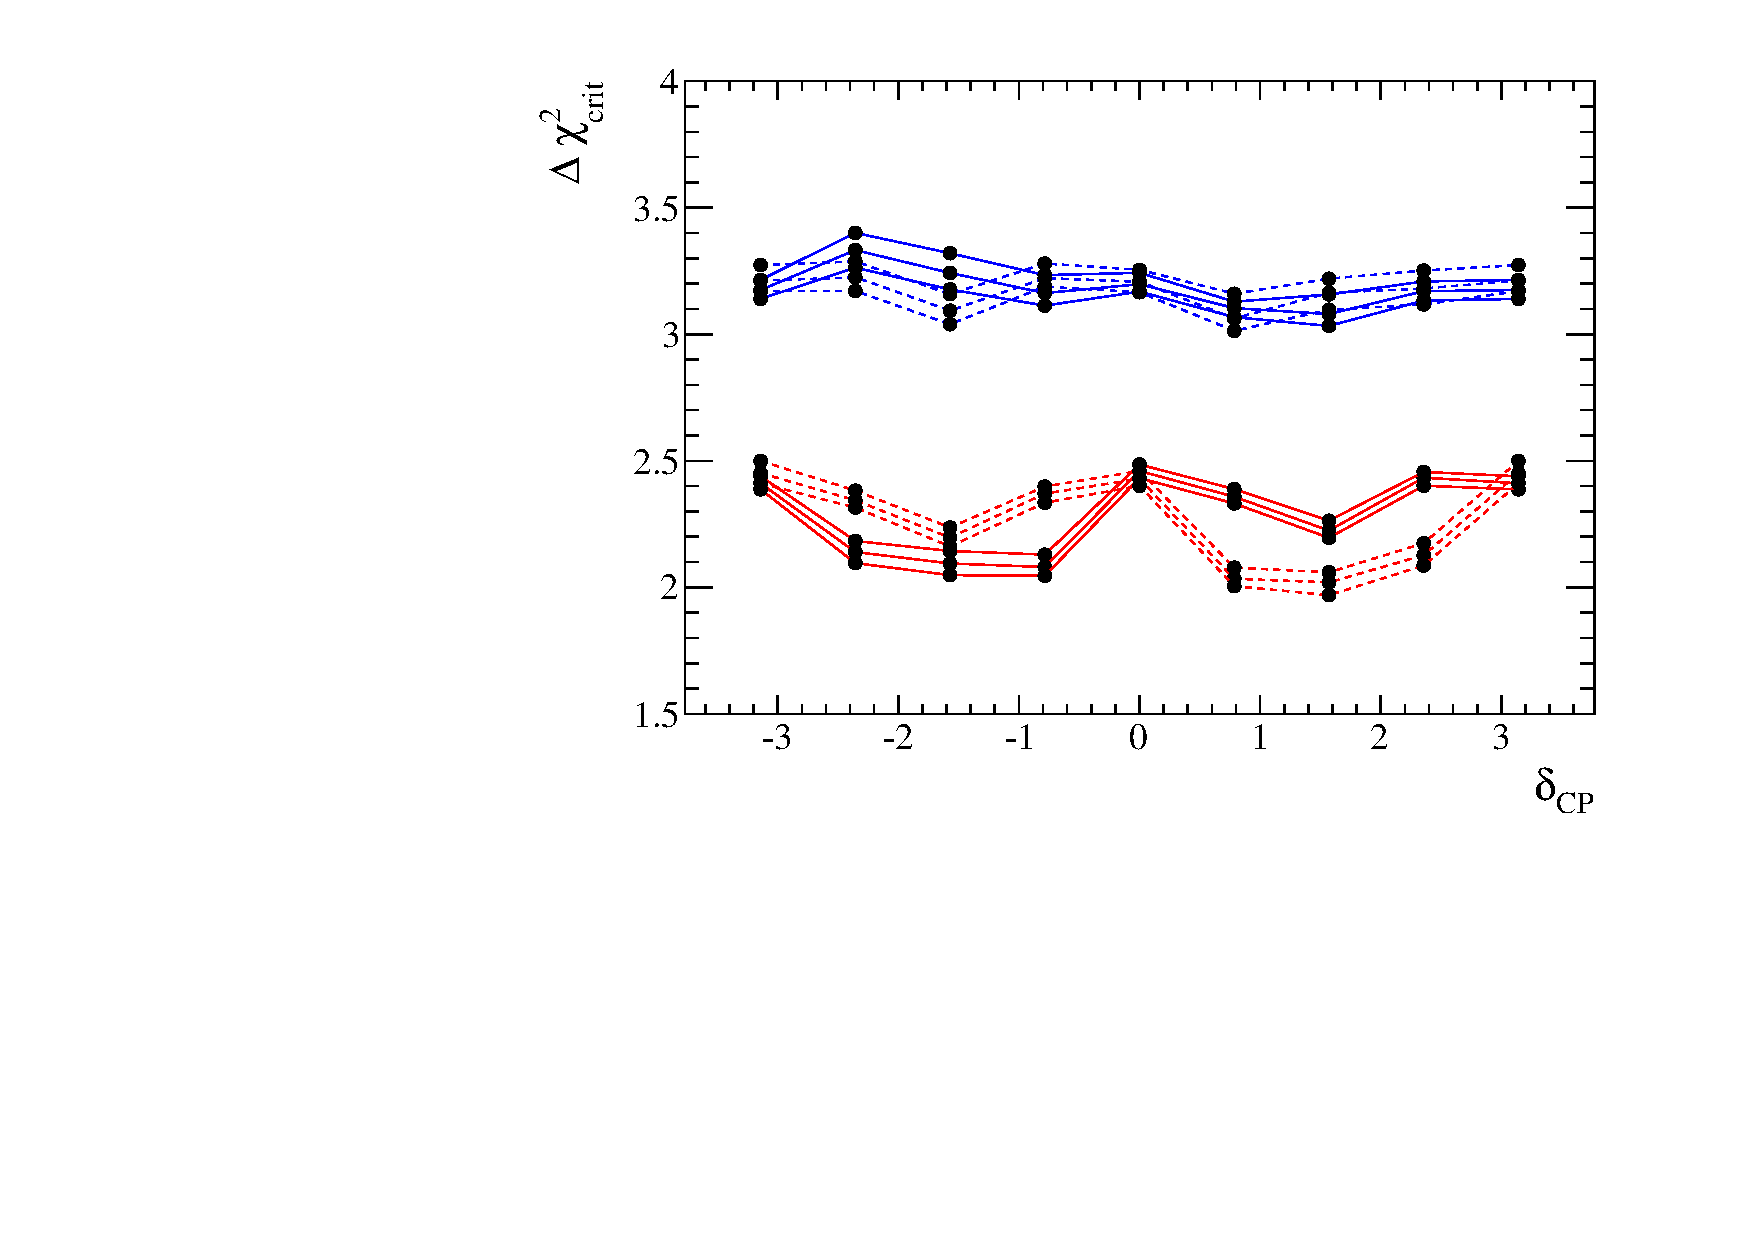
\includegraphics[width=0.9\textwidth]{./joint_plots/coverage_fc/fc/critical_values_Run16.pdf}
\caption{Critical values obtained with the Feldman-Cousins method for Run 1-6 statistic}
\end{subfigure}
\begin{subfigure}[b]{0.49\textwidth}
\includegraphics[width=0.9\textwidth]{./joint_plots/coverage_fc/fc_run17/critical_values_fluxrun16.pdf}
\caption{Critical values obtained with the Feldman-Cousins method for Run 1-7 statistic}
\end{subfigure}
\caption {
Critical values obtained with the Feldman-Cousins method for Run 1-6 and Run 1-7 statistic
for several true values of $\delta_{CP}$ and both normal (solid line) and inverted (dashed line) hierarchy.
Both 90\% (red) and $2\sigma$ (blue) CL critical values are shown.
About $10k$ toy experiments are performed for each point.
All the other oscillation parameters are marginalised.
The statistics corresponds to the Run 1-7 data set.
The $\pm1 \sigma$ error on the critical values is shown as well
and is represented by the lowest and highest set of critical values, with the same color of the central ones.
}
\label{fig:critval_comparision_run16_run17}
\end{figure*}


\clearpage





%
% Posterior predictive method
%

\subsection{Posterior predictive method for the choice of the prior}
\label{sec:posterior_predictive_run17}

The posterior predictive method has been tested for the Run 1-7 statistic as well
using the same procedure described in \cref{sec:posterior_predictive}.

As shown in \cref{tab:critval_posterior_Asimov_A_run17} and~\ref{tab:critval_posterior_Asimov_B_run17}
the posterior predictive critical values obtained for Asimov data sets A and B
at $1\sigma$, 90\% and $2\sigma$ CL are similar to the prior predictive ones,
as for the Run 1-6 statistic case.

\begin{figure*}[htb]
\center
\includegraphics[width=0.49\textwidth]{./joint_plots/coverage_fc/posterior_predictive_run17/Asimov_A/deltachisq_posterior_Asimov_A.pdf}
\caption {
$\Delta \chi^2$ distributions with prior (black) and posterior (red) predictive methods.
The comparison between the two distributions normalized to 1 is shown.
Fake data sets are generated with $\delta_{CP} = 0$ and normal hierarchy.
The Asimov data A is used to generate the weights of the fake data sets.
100k fake data sets are used.
Since the posterior predictive distribution is weighted, the effective number of entries is lower with respect 
to the prior predictive case. 
}
\label{fig:post_Asimov_A_dcp_0_nh_run17}
\end{figure*}


\begin{table}
\center
\begin{tabular}{| c | c | c |}
\hline
{\bf CL} 				& {\bf Prior} &{\bf Posterior}  \\
\hline
\hline
\multicolumn{3}{| c | }{$\delta^{true}_{CP} = 0$, $MH^{true} = \text{normal}$}  \\
\hline
$1\sigma$				&1.371  		& $1.308 ^{+0.014}_{-0.021}$	\\ \hline	
90\%					&2.601  		& $2.576 ^{+0.034}_{-0.020}$	\\ \hline	
$2\sigma$				&3.387 		& $3.351 ^{+0.067}_{-0.031}$	\\ \hline	
\hline
\multicolumn{3}{| c | }{$\delta^{true}_{CP} = 0$, $MH^{true} = \text{inverted}$}  \\
\hline
$1\sigma$				&1.346  		& $1.292 ^{+0.039}_{-0.021}$	\\ \hline	
90\%					&2.581  		& $2.565 ^{+0.052}_{-0.036}$	\\ \hline	
$2\sigma$				&3.381 		& $3.439 ^{+0.070}_{-0.063}$	\\ \hline	
\hline
\multicolumn{3}{| c | }{$\delta^{true}_{CP} = -1.351$, $MH^{true} = \text{inverted}$}  \\
\hline
$1\sigma$				&1.156   		& $ 1.132^{+0.019}_{-0.020}$	\\ \hline	
90\%					&2.318  		& $ 2.229^{+0.056}_{-0.035}$	\\ \hline	
$2\sigma$				&3.225 		& $ 3.046^{+0.095}_{-0.062}$	\\ \hline	
\end{tabular}
\caption{
The critical values of $\Delta \chi^2$ computed with Feldman-Cousins
for both prior and posterior predictive method are shown.
100k toy experiments were used for 
$\delta_{CP} = 0$ and normal hierarchy
and
about 50k toy experiments were used for 
$\delta_{CP} = 0$ and inverted hierarchy
and
$\delta_{CP} = -1.351$ and inverted hierarchy,
The weights of the fake data sets were generated with the Asimov data set A.
}             
\label{tab:critval_posterior_Asimov_A_run17}                                                                                                                                                                             
\end{table}


\begin{table}
\center
\begin{tabular}{| c | c | c |}
\hline
{\bf CL} 				& {\bf Prior} &{\bf Posterior}  \\
\hline
\hline
\multicolumn{3}{| c | }{$\delta^{true}_{CP} = 0$, $MH^{true} = \text{normal}$}  \\
\hline
$1\sigma$				&1.371  		& $1.299 ^{+0.013}_{-0.014}$	\\ \hline	
90\%					&2.601  		& $2.584 ^{+0.035}_{-0.019}$	\\ \hline	
$2\sigma$				&3.387 		& $3.445 ^{+0.035}_{-0.059}$	\\ \hline	
\hline
\multicolumn{3}{| c | }{$\delta^{true}_{CP} = 0$, $MH^{true} = \text{inverted}$}  \\
\hline
$1\sigma$				&1.346  		& $1.290 ^{+0.025}_{-0.015}$	\\ \hline	
90\%					&2.581  		& $2.531 ^{+0.033}_{-0.035}$	\\ \hline	
$2\sigma$				&3.381  		& $3.351 ^{+0.058}_{-0.080}$	\\ \hline	
\hline
\multicolumn{3}{| c | }{$\delta^{true}_{CP} = -1.351$, $MH^{true} = \text{inverted}$}  \\
\hline
$1\sigma$				&1.15568  	& $ 1.132^{+0.015}_{-0.019}$	\\ \hline	
90\%					& 2.31821 	& $2.318 ^{+0.048}_{-0.050}$	\\ \hline	
$2\sigma$				& 3.22547		& $3.238 ^{+0.065}_{-0.062}$	\\ \hline	
\end{tabular}
\caption{
The critical values of $\Delta \chi^2$ computed with Feldman-Cousins
for both prior and posterior predictive method are shown.
100k toy experiments were used for
$\delta_{CP} = 0$ and normal hierarchy
and
about 50k toy experiments were used for 
$\delta_{CP} = 0$ and inverted hierarchy
and
$\delta_{CP} = -1.351$ and inverted hierarchy,
The weights of the fake data sets were generated with the Asimov data set B.
}             
\label{tab:critval_posterior_Asimov_B_run17}                                                                                                                                                                             
\end{table}


\clearpage




%
% Validation minimization algorithm
%

\subsection{Validation of the minimization algorithm}
\label{sec:minim_algorithm_run17}

The minimization algorithm has been tested for the Run 1-7 statistic as well.
Analogue results as already shown in \cref{sec:minim_algorithm} are obtained.
For each true value of $\delta_{CP}$, where the critical value is performed using the Feldman-Cousins method,
and normal hierarchy, 500 fits were performed on fake data sets of the same type as used for Feldman-Cousins.
All the fits found the global minimum.



\clearpage

